\section{Priority scheduling and prefix estimates}
\label{sec:foundations-rounding}

Choose a single $\alpha$ uniformly from $(0,1)$ and assign each original
job $i$ the key $M_i(\alpha)$. Write $\mathbb E[X]$ for the expectation of
$X$ over this choice of $\alpha$.
Resolve equal keys by increasing job number. At the beginning of each integer slot,
schedule the $\min\{m,\text{number of ready jobs}\}$ ready original jobs
with smallest keys, using this tie order. A job is \emph{ready} if it has not
yet been scheduled and all its predecessors have completed. Every scheduled
job occupies the whole slot.
A rule that schedules as many ready jobs as possible in each slot is called
\emph{non-delay}. This machine-driven list rule is
feasible and finishes in at most $n$ slots: whenever original jobs remain,
a minimal unfinished original job is ready. Virtual jobs are used only in
the analysis and are never scheduled. The complete deterministic algorithm
is summarized below. Its polynomial implementation is proved in
Section~\ref{sec:foundations-derandomization}.

We represent a feasible integer-slot schedule by its completion-time vector.
Within each slot, assign jobs in increasing job order to machines in increasing
order. For a set of ready jobs,
$\operatorname{first}_k$ returns its first $k$ members in increasing order
of $M_j(\alpha)$, with ties broken by increasing job number.
An isolated zero has a neighborhood containing no other zeros. In the
return statement, $\operatorname*{arg\,min}$ selects the lexicographically
first minimizing vector, comparing vectors at their first differing coordinate.
Use a fixed deterministic polynomial-time LP algorithm to choose a rational
optimal solution in the step below.

\begin{algorithm}[H]
\DontPrintSemicolon
\caption{Deterministic common-quantile scheduling}
\label{alg:rounding}
\KwIn{$\mathcal O$, the precedence relation, $(w_j)_{j\in\mathcal O}$, $m$}
\KwOut{A feasible completion-time vector}
\If{$m\ge n$}{\KwRet{$(a_j)_{j\in\mathcal O}$}\;}
Compute an optimal LP solution $(x_{i,s})_{i\in\mathcal O,\,1\le s\le n}$\;
$\mathcal C\gets\{0,1\}\cup
  \bigl\{F_i(s):i\in\mathcal O,\ 1\le s\le n\bigr\}$\;
$\mathcal C\gets\mathcal C\cup
  \bigl\{\alpha\in(0,1):\text{$\alpha$ is an isolated zero of $M_i-M_k$ for
  some distinct $i,k\in\mathcal O$}\bigr\}$\;
$\mathcal S\gets\varnothing$\;
\ForEach{consecutive $\alpha_-<\alpha_+$ in $\mathcal C$}{
  $\alpha\gets(\alpha_-+\alpha_+)/2$\;
  $\mathcal W\gets\mathcal O$\;
  $s\gets1$\;
  \While{$\mathcal W\ne\varnothing$}{
    $\mathcal U\gets\{j\in\mathcal W:\{i\in\mathcal O:i\to j\}\cap\mathcal W=\varnothing\}$\;
    $\mathcal V\gets\operatorname{first}_{\min\{m,|\mathcal U|\}}(\mathcal U)$\;
    $(C_j)_{j\in\mathcal V}\gets(s)_{j\in\mathcal V}$\;
    $\mathcal W\gets\mathcal W\setminus\mathcal V$\;
    $s\gets s+1$\;
  }
  $\mathcal S\gets\mathcal S\cup\{(C_j)_{j\in\mathcal O}\}$\;
}
\KwRet{$\displaystyle\operatorname*{arg\,min}_{(C_j)_{j\in\mathcal O}\in\mathcal S}
                  \sum_{j\in\mathcal O}w_j\cdot C_j$}\;
\end{algorithm}

The completed jobs form a predecessor-closed set, so checking incoming arcs
suffices to identify ready jobs. The set $\mathcal U$ is nonempty whenever
$\mathcal W$ is nonempty because the precedence graph is acyclic.
If two jobs' quantile functions agree throughout an interval,
increasing job number resolves their tie and no extra breakpoint is
needed. Section~\ref{sec:foundations-derandomization} proves polynomial
running time and bounds the cost returned by Algorithm~\ref{alg:rounding}.


Fix an original target $j$ and a parameter $\alpha$. Define
\[
 \mathcal J_\alpha=\{i\in\mathcal J:M_i(\alpha)\le M_j(\alpha)\}.
\]
The original prefix $\mathcal J_\alpha\cap\mathcal O$ includes all original jobs tied with
$j$, including those later in the fixed tie order. It is predecessor
closed by \eqref{eq:foundations-quantile-separation}.

\begin{lemma}[Restriction to a priority prefix]
Running the priority rule only on $\mathcal J_\alpha\cap\mathcal O$ gives the same completion
times for its jobs as running it on all original jobs.
\end{lemma}
\begin{proof}
Induct on slots. The ready jobs in $\mathcal J_\alpha\cap\mathcal O$ agree in the two runs.
They all have higher priority than original jobs outside $\mathcal J_\alpha\cap\mathcal O$,
and the latter jobs can only fill unused places in the current slot.
As processing times are one, these outside jobs reserve no capacity in
subsequent slots.
\end{proof}

Let $\widetilde C_j(\alpha)$ be the target's actual completion time.
A slot is \emph{underfull} if fewer than $m$ jobs run in it. Let
$N_j(\alpha)$ count underfull slots through the target's completion in
the schedule restricted to $\mathcal J_\alpha\cap\mathcal O$.

The following prefix estimate adapts Li's workload and depth argument to
our priority rule \cite[Lemma~3.2]{Li2017}.

\begin{lemma}[Workload and height bounds]
\label{lem:prefix-work-height}
For the restricted schedule,
\[
 \widetilde C_j(\alpha)\le |\mathcal J_\alpha\cap\mathcal O|/m+N_j(\alpha),
 \qquad N_j(\alpha)\le a_j.
\]
\end{lemma}
\begin{proof}
The first inequality counts fully occupied slots, each using $m$
distinct original prefix jobs. For the second, consider the set of
unfinished predecessors of $j$, including $j$ if it is unfinished.
We call this the \emph{unfinished ancestor set} of $j$. It is predecessor closed
within the unfinished jobs. In an underfull slot every ready prefix job
executes, so all minimal jobs of this set execute and its height decreases
by at least one.
Its initial height is $a_j$, and it never increases. This includes
the slot in which $j$ finishes.
\end{proof}

To preserve the exact-capacity scalar identities, define the analytical
\emph{prefix correction}
\[
 I_j(\alpha):=N_j(\alpha)-|\mathcal J_\alpha\cap\mathcal D|/m.
\]
When $\alpha$ is random, we omit its argument from $I_j$ and
$\widetilde C_j$.
The prefix correction may be negative or nonintegral. It is not an underfull-slot
count. Its purpose is to credit the virtual prefix work that the actual
scheduler never executes. The preceding estimates give
\begin{equation}
 \widetilde C_j(\alpha)\le |\mathcal J_\alpha|/m+I_j(\alpha),
 \qquad I_j(\alpha)\le a_j.
 \label{eq:foundations-prefix-bound}
\end{equation}
The priority-band lemma below is first proved for the actual underfull
count. Proposition~\ref{prop:virtual-pool-transfer} then shows that its
weighted conclusion applies to $I_j$ with the full virtual pool.

Following Li's scalar reduction \cite[Section~3]{Li2017}, write
$h_i(\alpha)=F_i(M_j(\alpha))$ for every original or virtual job. Each
$h_i$ is nondecreasing and measurable because $F_i$ is continuous and
$M_j$ is nondecreasing. Then
\begin{equation}
 |\mathcal J_\alpha|=\sum_{i\in\mathcal J}
       \mathbf1\{h_i(\alpha)\ge\alpha\},\qquad
 \sum_{i\in\mathcal J}h_i(\alpha)=m\cdot M_j(\alpha).
 \label{eq:foundations-h-identities}
\end{equation}
The first identity follows from the quantile definition and continuity
of the CDFs. The second follows from the exact capacity provided by our
padding in \eqref{eq:foundations-continuous-capacity}. No virtual-job priority need be
computed by the algorithm.
\section{Scalar area and excess}
\label{sec:meta-scalar}

Write $c=\sqrt2-1$, so $c+2=1+\sqrt2$ and $(c+2)\cdot c=1$.
For a real number $x$, let $(x)_+=\max\{x,0\}$.
The next lemma refines Li's scalar bound \cite[Claim 3.3]{Li2017} by
retaining the area above the baseline. We include the proof and the exact
identities needed below.

Let $h:[0,1]\to[0,1]$ be nondecreasing and measurable. Define
\[
 u=h(0),\qquad \beta=|\{z\in[0,1]:h(z)\ge z\}|.
\]
The \emph{excess} and \emph{deficit} are
\[
 \zeta=\int_0^1h(z)\,dz-\frac{u^2}{2}-\beta+\frac{\beta^2}{2},
 \qquad
 f(u,\beta)=(c+2)\cdot\left(\frac{u^2}{2}+\beta-\frac{\beta^2}{2}\right)-u-\beta.
\]

\begin{lemma}[Scalar area and excess]
\label{lem:meta-scalar-area}
We have $0\le u\le\beta\le1$ and
\[
 \zeta\ge\int_0^1(h(z)-\max\{u,z\})_+\,dz\ge0.
\]
The deficit $f(u,\beta)$ is nonnegative and satisfies
\begin{align}
 f(u,\beta)&=\frac{c+2}{2}\cdot(u-c\cdot\beta)^2+(1-\beta)\cdot((c+1)\cdot\beta-u)\ge0,
 \label{eq:meta-f-nonnegative}\\
 f(u,\beta)&=\frac{c+2}{2}\cdot\bigl[(u-c)^2+(1-\beta)\cdot(\beta-c^2)\bigr].
 \label{eq:meta-f-square}
\end{align}
Also, for every $z\in[0,1]$,
\[
 h(z)\ge\max\{u,z-(1-\beta)\}.
\]
\end{lemma}
\begin{proof}
Let $\mathcal N=\{z\in[0,1]:h(z)<z\}$. Its measure is $1-\beta$.
Since $h\ge u$, we have $h(z)\ge z$ for $z\in[0,u]$, so $u\le\beta$.
For $z\in\mathcal N$, monotonicity gives $(h(z),z]\subseteq\mathcal N$.
Thus $z-h(z)\le |\mathcal N\cap[0,z]|$.
The second integral in the next display counts the area of pairs $(x,z)\in\mathcal N^2$ with
$x\le z$. Swapping the coordinates exchanges this region with its
complement in $\mathcal N^2$, apart from the diagonal, which has area zero.
Thus the region has half the area of $\mathcal N^2$, and
\[
 \int_{\mathcal N}(z-h(z))\,dz\le
 \int_{\mathcal N}|\mathcal N\cap[0,z]|\,dz
 = (1-\beta)^2/2.
\]
The decomposition
\begin{align*}
 \int_0^1h(z)\,dz
 &=\underbrace{\frac{1+u^2}{2}}_{\text{baseline area}}
   +\underbrace{\int_0^1(h(z)-\max\{u,z\})_+\,dz}_{\text{excess above the baseline}}\\
 &\quad-\underbrace{\int_{\mathcal N}(z-h(z))\,dz}_{\text{shortfall below the diagonal}}\\
 &\ge\frac{u^2}{2}+\beta-\frac{\beta^2}{2}
      +\int_0^1(h(z)-\max\{u,z\})_+\,dz
\end{align*}
proves the excess statement. The two identities follow by expansion
using $(c+2)\cdot c=1$ and $c^2+2\cdot c=1$. The second term in
\eqref{eq:meta-f-nonnegative} is nonnegative because $u\le\beta$
and $c+1>1$. Finally, if $h(z)<z$, the interval $(h(z),z]$ has
measure at most $1-\beta$, proving the last assertion. The other case
and the lower bound $h\ge u$ are immediate.
\end{proof}

Li already identified the nonzero extremal profile below
\cite[Section~3]{Li2017}. Its connection to the priority band motivates
our refinement. If
$f(u,\beta)=0$ and $\zeta=0$, the first identity and $u\le\beta$ give
$\beta\in\{0,1\}$. If $\beta=0$, then $u=0$ and $h=0$ almost everywhere.
If $\beta=1$, then $u=c$. Since $h(z)\ge\max\{c,z\}$ almost everywhere
and $\zeta=0$, the excess bound gives $h(z)=\max\{c,z\}$ almost everywhere.

\section{Progress forced by a priority band}
The following structural statements concern an arbitrary non-delay priority
list schedule of unit jobs and its underfull-slot counts $N_j$. The idea is that a scheduled job with a late key cannot
occupy a machine while an earlier-key job is ready but unscheduled. A sequence of slots
containing late-key jobs therefore removes layers of early-key predecessors
of the target, even when those slots are full. Figure~\ref{fig:band-progress}
shows an example.
\begin{figure}[tb]
\centering
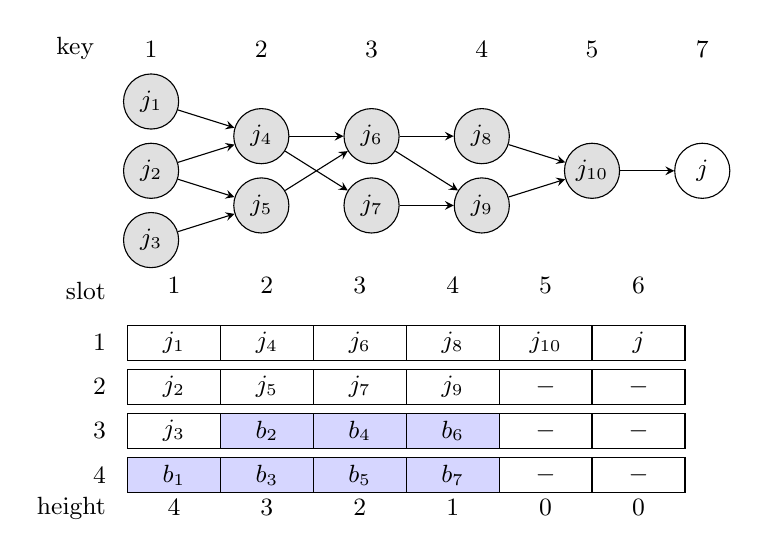
\begin{tikzpicture}[x=1cm,y=.8cm,>=stealth,font=\small,
  job/.style={circle,draw,fill=black!12,minimum size=7mm,inner sep=0pt},
  target/.style={circle,draw,minimum size=7mm,inner sep=0pt}]
  % The early-ancestor DAG. Numbers above columns are priority keys.
  \node[job] (a) at (.3,1.1) {$j_1$};
  \node[job] (b) at (.3,0) {$j_2$};
  \node[job] (c) at (.3,-1.1) {$j_3$};
  \node[job] (d) at (1.7,.55) {$j_4$};
  \node[job] (e) at (1.7,-.55) {$j_5$};
  \node[job] (f) at (3.1,.55) {$j_6$};
  \node[job] (g) at (3.1,-.55) {$j_7$};
  \node[job] (h) at (4.5,.55) {$j_8$};
  \node[job] (i) at (4.5,-.55) {$j_9$};
  \node[job] (k) at (5.9,0) {$j_{10}$};
  \node[target] (j) at (7.3,0) {$j$};
  \foreach \from/\to in {a/d,b/d,b/e,c/e,d/f,e/f,d/g,f/h,f/i,g/i,h/k,i/k,k/j}
    \draw[->] (\from)--(\to);
  \foreach \x/\key in {.3/1,1.7/2,3.1/3,4.5/4,5.9/5,7.3/7}
    \node[above] at (\x,1.65) {$\key$};
  \node[anchor=east] at (-.3,1.95) {key};
  % Rows are machines and columns are slots.
  \foreach \x/\slot in {0/1,1.18/2,2.36/3,3.54/4,4.72/5,5.90/6}
    \node[above] at (\x+.59,-2.1) {$\slot$};
  \node[anchor=east] at (-.15,-1.9) {slot};
  \foreach \y/\machine in {-2.45/1,-3.15/2,-3.85/3,-4.55/4}
    \node[anchor=east] at (-.15,\y-.28) {$\machine$};
  \node[anchor=east] at (-.15,-5.35) {height};
  \foreach \x/\one/\two/\three/\four in {
    0/j_1/j_2/j_3/b_1,
    1.18/j_4/j_5/b_2/b_3,
    2.36/j_6/j_7/b_4/b_5,
    3.54/j_8/j_9/b_6/b_7,
    4.72/j_{10}/{-}/{-}/{-},
    5.90/j/{-}/{-}/{-}}
  {
    \foreach \y/\entry in {-2.45/\one,-3.15/\two,-3.85/\three,-4.55/\four}
    {
      \draw (\x,\y) rectangle ++(1.18,-.56);
      \node at (\x+.59,\y-.28) {$\entry$};
    }
  }
  \foreach \x/\y/\entry in {
    0/-4.55/b_1,1.18/-3.85/b_2,1.18/-4.55/b_3,
    2.36/-3.85/b_4,2.36/-4.55/b_5,
    3.54/-3.85/b_6,3.54/-4.55/b_7}
  {
    \fill[blue!16] (\x,\y) rectangle ++(1.18,-.56);
    \draw (\x,\y) rectangle ++(1.18,-.56);
    \node at (\x+.59,\y-.28) {$\entry$};
  }
  \foreach \x/\height in {0/4,1.18/3,2.36/2,3.54/1,4.72/0,5.90/0}
    \node at (\x+.59,-5.35) {$\height$};
\end{tikzpicture}
\caption{A priority-band example with four machines. The graph shows the
predecessors of the target $j$ and their precedence arcs. The number
above each column is the priority key. The seven independent jobs
$b_1,\ldots,b_7$ have depth one and key $6$. The jobs are numbered in the
order $j_1,\ldots,j_{10},j,b_1,\ldots,b_7$. With threshold $5.9$, the
$b_i$ lie in the priority band $(5.9,7]$. The table gives a non-delay priority schedule.
Each of its first four slots is full and contains a band job. Its final row
shows the height of the unfinished early-key predecessors after each slot,
starting from height five. The band slots force this height to fall to one
even though no machine is idle. Dashes denote idle machines.}
\label{fig:band-progress}
\end{figure}


Fix a target $j$ and a real threshold $t$. Let $\mathcal I$ be the
set of predecessors of $j$ with key at most $t$.

\begin{lemma}[Early-predecessor progress]
\label{lem:early-ancestor-progress}
Suppose keys increase by at least one along each precedence edge.
After $k$ slots each containing a job with key greater than $t$,
the unfinished part of $\mathcal I$ has height at most $(a_j-1-k)_+$.
\end{lemma}
\begin{proof}
The set $\mathcal I$ is predecessor closed and has height at most $a_j-1$. In
each specified slot, every ready job of $\mathcal I$ is scheduled: otherwise it
would have priority over the scheduled job with key greater than $t$.
Consequently all minimal unfinished members of $\mathcal I$ are removed, and
its height falls by at least one whenever it is nonempty.
\end{proof}

\begin{lemma}[Counting keys on a chain]
\label{lem:chain-in-band}
Let $t<t'$. If consecutive keys on a chain differ by at least one, the number of
its jobs with keys in $(t,t']$ is at most $\lceil t'-t\rceil$.
\end{lemma}
\begin{proof}
If there are no such jobs, the claim is immediate because $t<t'$.
Otherwise, if there are $k$ such jobs, then $k-1<t'-t$. Since $k$ is an
integer, the result follows.
\end{proof}

Fix $0<\kappa<\alpha<1$ and consider a non-delay priority list schedule of
unit jobs on $m$ machines. Its keys satisfy $M_r(\alpha)\ge M_i(\alpha)+1$ on every precedence arc
$i\to r$. Fix a target $j$ of depth $a_j$ and restrict
to all jobs of key at most $M_j(\alpha)$, retaining every tie. Let $N_j(\alpha)$ be the
number of underfull integer slots through the target's completion in
this restricted schedule. The schedule continues until every job in the
prefix has completed.

Continuity gives $F_j(M_j(\alpha-\kappa))=\alpha-\kappa$ and
$F_j(M_j(\alpha))=\alpha$. Since $M_j$ is nondecreasing,
$M_j(\alpha-\kappa)<M_j(\alpha)$. Let $d_0\ge0$ and let $\mathcal K$
be a set of jobs of depth at most $d_0$ whose keys lie in
$(M_j(\alpha-\kappa),M_j(\alpha)]$.

\begin{lemma}[Priority-band bound]
Then
\begin{equation}
 N_j(\alpha)\le d_0+(a_j-|\mathcal K|/m)_++M_j(\alpha)-M_j(\alpha-\kappa).
 \label{eq:priority-band}
\end{equation}
\end{lemma}

\begin{proof}
We use the height argument from Lemma~\ref{lem:prefix-work-height}:
at a slot boundary, the height of the unfinished ancestor set bounds the
number of subsequent underfull slots through the target completion.

Assume $\mathcal K$ is nonempty. Let $s^*$ be the latest completion slot
of any job in $\mathcal K$, and choose a job $i\in\mathcal K$ completing at
$s^*$. At least $\lceil|\mathcal K|/m\rceil$ distinct slots contain a job
of $\mathcal K$. Let $\mathcal I$ be the predecessors of $j$ whose keys are
at most $M_j(\alpha-\kappa)$. At the start of slot $s^*$, at least
$\lceil|\mathcal K|/m\rceil-1$ earlier slots containing jobs of $\mathcal K$
have occurred. By
Lemma~\ref{lem:early-ancestor-progress}, the remaining height of $\mathcal I$
is at most $(a_j-\lceil|\mathcal K|/m\rceil)_+$.

Any chain in the unfinished ancestor set of $j$ at the start of $s^*$
splits into an initial segment with key at most $M_j(\alpha-\kappa)$ and a terminal
segment with key greater than $M_j(\alpha-\kappa)$. The former has length at most
$(a_j-\lceil|\mathcal K|/m\rceil)_+$. By Lemma~\ref{lem:chain-in-band}, the terminal segment
has at most $\lceil M_j(\alpha)-M_j(\alpha-\kappa)\rceil$ jobs. The whole remaining ancestor height is therefore
at most
\[
 (a_j-\lceil|\mathcal K|/m\rceil)_++\lceil M_j(\alpha)-M_j(\alpha-\kappa)\rceil.
\]

Before slot $s^*$, at most $a_i-1$ slots are underfull. Each such slot
decreases the height of the unfinished ancestor set of $i$, which still
contains $i$ at the start of slot $s^*$. From slot $s^*$ through $j$'s
completion, the number of underfull slots is at most the displayed height
bound. If $j$ has already completed, there are no such slots. Therefore,
using $a_i\le\lfloor d_0\rfloor$,
\[
 N_j(\alpha)\le\lfloor d_0\rfloor+(a_j-\lceil|\mathcal K|/m\rceil)_+
 +\lceil M_j(\alpha)-M_j(\alpha-\kappa)\rceil-1.
\]
Since $(a_j-\lceil|\mathcal K|/m\rceil)_+\le(a_j-|\mathcal K|/m)_+$ and
$\lceil M_j(\alpha)-M_j(\alpha-\kappa)\rceil-1\le M_j(\alpha)-M_j(\alpha-\kappa)$, this proves \eqref{eq:priority-band}
when $\mathcal K$ is nonempty. If $\mathcal K$ is empty, the bound follows
directly from $N_j(\alpha)\le a_j$, as
$d_0\ge0$ and $M_j(\alpha)>M_j(\alpha-\kappa)$.
\end{proof}

For the original-only scheduler, assign each job $i\in\mathcal J$ a
fixed weight $\theta_i\in[0,1]$. Suppose
$\sum_{i\in\mathcal J}\theta_i\ge m\cdot(a_j-1)$ and each positive-weight
original job has depth at most $d_0\ge0$.

\begin{proposition}[Virtual-pool transfer]
\label{prop:virtual-pool-transfer}
The prefix correction satisfies
\[
\begin{aligned}
 a_j-I_j(\alpha)\ge{}&
 a_j-1-d_0-M_j(\alpha)+M_j(\alpha-\kappa)\\
 &-\frac1m\cdot\sum_{\substack{i\in\mathcal J\\
 M_i(\alpha)\notin(M_j(\alpha-\kappa),M_j(\alpha)]}}\theta_i.
\end{aligned}
\]
\end{proposition}
\begin{proof}
Let $\mathcal K$ be the positive-weight original jobs with keys in the
band. Applying the priority-band bound gives
\[
 a_j-N_j(\alpha)\ge
 \min\left\{a_j,\frac{|\mathcal K|}{m}\right\}
 -d_0-M_j(\alpha)+M_j(\alpha-\kappa).
\]
Each virtual job in the band lies in $\mathcal J_\alpha\cap\mathcal D$.
Since each weight is at most one,
\[
 \sum_{\substack{i\in\mathcal J\\
 M_i(\alpha)\in(M_j(\alpha-\kappa),M_j(\alpha)]}}\theta_i
 \le |\mathcal K|+|\mathcal J_\alpha\cap\mathcal D|.
\]
Thus
\begin{align*}
 &\min\left\{a_j,\frac{|\mathcal K|}{m}\right\}
 +\frac{|\mathcal J_\alpha\cap\mathcal D|}{m}\\
 &\quad\ge\min\left\{a_j,\frac1m\cdot\sum_{\substack{i\in\mathcal J\\
 M_i(\alpha)\in(M_j(\alpha-\kappa),M_j(\alpha)]}}\theta_i\right\}\\
 &\quad\ge a_j-1-\frac1m\cdot\sum_{\substack{i\in\mathcal J\\
 M_i(\alpha)\notin(M_j(\alpha-\kappa),M_j(\alpha)]}}\theta_i.
\end{align*}
For the last step, both terms in the minimum are at least the displayed
lower bound, by the assumed total pool weight and nonnegativity of the weights.
Adding the virtual-prefix credit $|\mathcal J_\alpha\cap\mathcal D|/m$ to
the first bound and using the definition of $I_j(\alpha)$ proves the claim.
\end{proof}
\section{A partial pool with automatic feasibility}
\label{sec:meta-pool}

Fix an original target $j$.
Extend each $h_i$ to $[0,1]$ by setting $h_i(0)$ and $h_i(1)$ to its
respective one-sided limits. These limits exist because $h_i$ is nondecreasing and
bounded. Values at the endpoints do not affect the integrals below. Let
$u_i,\beta_i,\zeta_i$ be the resulting scalar quantities and set
$f_i=f(u_i,\beta_i)$. The expected size of the
full padded prefix, divided by $m$, is $m^{-1}\cdot\sum_{i\in\mathcal J}\beta_i$. Exact capacity
and the quantile mean imply
\begin{align*}
 \sum_{i\in\mathcal J}u_i&=m\cdot M_j(0),\\
 \frac1m\cdot\sum_{i\in\mathcal J}\beta_i
 &=(c+2)\cdot(C_j^{\mathrm{LP}}-1/2)-M_j(0)
   -\frac1m\cdot\sum_{i\in\mathcal J}(f_i+(c+2)\cdot\zeta_i).
\end{align*}
Every summand in the final sum is nonnegative by
Lemma~\ref{lem:meta-scalar-area}.
Indeed, \eqref{eq:foundations-h-identities} gives
$\sum_{i\in\mathcal J} h_i(\alpha)=m\cdot M_j(\alpha)$, including in the limit
$\alpha\downarrow0$. The definition of $f_i$ gives
$\beta_i=(c+2)\cdot(\int_0^1h_i(\alpha)\,d\alpha-\zeta_i)-u_i-f_i$.
Summing and using the quantile mean \eqref{eq:foundations-quantile-mean}
proves the displayed identity for the expected prefix size.
The prefix correction from \eqref{eq:foundations-prefix-bound}
satisfies $I_j\le a_j$ and
$\mathbb E[\widetilde C_j]\le\frac1m\cdot\sum_{i\in\mathcal J}\beta_i+\mathbb E[I_j]$. Therefore
\begin{equation}
\begin{aligned}
 (c+2)\cdot C_j^{\mathrm{LP}}-\mathbb E[\widetilde C_j]
 &\ge\frac1m\cdot\sum_{i\in\mathcal J}(f_i+(c+2)\cdot\zeta_i)\\
 &\quad +(M_j(0)-a_j+1)+c/2+\mathbb E[a_j-I_j].
\end{aligned}
 \label{eq:meta-gap-identity}
\end{equation}

Choose $0<U<1$ and define the \emph{time cutoff}
\begin{equation}
 d=U\cdot(a_j-1)+\frac1m\cdot\sum_{i\in\mathcal J}(u_i-U)_+.
 \label{eq:meta-automatic-cut}
\end{equation}
Define the pool weights by
\[
 \theta_i=\min\{F_i(d)/U,1\}\qquad(i\in\mathcal J).
\]

\begin{lemma}[Feasibility and size of the partial pool]
\label{lem:partial-pool}
The cutoff \eqref{eq:meta-automatic-cut} satisfies $0\le d\le M_j(0)$ and
$\sum_{i\in\mathcal J}\theta_i\ge m\cdot(a_j-1)$. Every positive-weight original pool job has
depth at most $d+1$, and $\theta_i\le\min\{u_i/U,1\}$ for every job.
\end{lemma}
\begin{proof}
The cutoff is automatically feasible: $(u-U)_+\le(1-U)\cdot u$ for
$0\le u\le1$, so
\[
 0\le d\le U\cdot(a_j-1)+(1-U)\cdot M_j(0)\le M_j(0).
\]
These pool weights are unrelated to the objective weights. Since
$d\le M_j(0)$, monotonicity and continuity give $F_i(d)\le F_i(M_j(0))=u_i$.
Exact capacity gives
\[
 \sum_{i\in\mathcal J}\theta_i=\frac{m\cdot d-\sum_{i\in\mathcal J}(F_i(d)-U)_+}{U}
 \ge\frac{m\cdot d-\sum_{i\in\mathcal J}(u_i-U)_+}{U}=m\cdot(a_j-1).
\]
An original job of depth $a_i$ has no interpolated mass at or before
$a_i-1$. Thus every positive-weight original pool job has
$a_i-1<d$, and hence depth at most $d+1$. Also
$\theta_i\le\min\{u_i/U,1\}$.
\end{proof}

Choose a quantile band with
\begin{equation}
 0<\kappa<\ell\le1-\kappa,\qquad U\le\ell.
 \label{eq:meta-band-domain}
\end{equation}
In particular, $\kappa<1/2$ and $\ell<1$.
At quantile $\alpha\in[\ell,1)$
the priority band is $(M_j(\alpha-\kappa),M_j(\alpha)]$.
Define job $i$'s integrated weighted failure to lie in this band by
\[
 \mathcal F_i=\theta_i\cdot\left|\left\{\alpha\in[\ell,1):
 M_i(\alpha)\notin(M_j(\alpha-\kappa),M_j(\alpha)]\right\}\right|,
\]
where the fixed pool weight $\theta_i$ is as in Lemma~\ref{lem:partial-pool}.
The two ways to fail are disjoint: the key lies at most at the lower
endpoint, or strictly above the upper endpoint. For a nondecreasing function
$h$, write its integrated movement across the band as
\[
 \mathcal M(h)=\int_\ell^1
           [h(\alpha)-h(\alpha-\kappa)]\,d\alpha.
\]
Changing variables in the second integral and canceling the common part gives
\[
 \mathcal M(h)=\int_{1-\kappa}^{1}h(x)\,dx
 -\int_{\ell-\kappa}^{\ell}h(x)\,dx.
\]
For $\alpha\in[\ell,1)$, continuity of the CDFs gives the
exact event equivalences
\[
 \begin{aligned}
 M_i(\alpha)>M_j(\alpha)
   &\ \Longleftrightarrow\ h_i(\alpha)<\alpha,\\
 M_i(\alpha)\le M_j(\alpha-\kappa)
   &\ \Longleftrightarrow\ h_i(\alpha-\kappa)\ge\alpha.
 \end{aligned}
\]
These identities connect the subsequent
scalar estimates to the actual quantile priorities.
\begin{lemma}[Integrated progress from the partial pool]
\label{lem:integrated-partial-pool}
The quantities just defined satisfy
\begin{equation}
 \mathbb E[a_j-I_j]\ge (1-\ell)\cdot\bigl((1-U)\cdot a_j-2+U\bigr)
 -\frac1m\cdot\sum_{i\in\mathcal J}\left[(1-\ell)\cdot(u_i-U)_++\mathcal F_i+\mathcal M(h_i)\right].
 \label{eq:meta-complete-loss}
\end{equation}
\end{lemma}
\begin{proof}
For $\alpha\in[\ell,1)$, apply
Proposition~\ref{prop:virtual-pool-transfer} with the weights above and
$d_0=d+1$. Its hypotheses hold by Lemma~\ref{lem:partial-pool}. Thus
\[
 a_j-I_j(\alpha)\ge a_j-2-d-
 \bigl(M_j(\alpha)-M_j(\alpha-\kappa)\bigr)
 -\frac1m\cdot\sum_{\substack{i\in\mathcal J\\
 M_i(\alpha)\notin(M_j(\alpha-\kappa),M_j(\alpha)]}}\theta_i.
\]
Integrate over $[\ell,1]$. Since $\sum_{i\in\mathcal J} h_i(\alpha)=m\cdot M_j(\alpha)$,
\begin{align*}
 \int_\ell^1\!\bigl(M_j(\alpha)-M_j(\alpha-\kappa)\bigr)\,d\alpha
 &=\frac1m\cdot\sum_{i\in\mathcal J}\mathcal M(h_i),\\
 \int_\ell^1\sum_{\substack{i\in\mathcal J\\
 M_i(\alpha)\notin(M_j(\alpha-\kappa),M_j(\alpha)]}}\theta_i\,d\alpha
 &=\sum_{i\in\mathcal J}\mathcal F_i.
\end{align*}
The second identity follows from the definition of $\mathcal F_i$.
For quantiles below $\ell$, we have $a_j-I_j\ge0$, so integration over
$[\ell,1]$ lower bounds its expectation. Substituting the definition of $d$ gives
\eqref{eq:meta-complete-loss}.
\end{proof}
